\documentclass[tikz,border=6pt]{standalone}
\usepackage{amsmath}
\usetikzlibrary{arrows.meta,calc,positioning}

\begin{document}
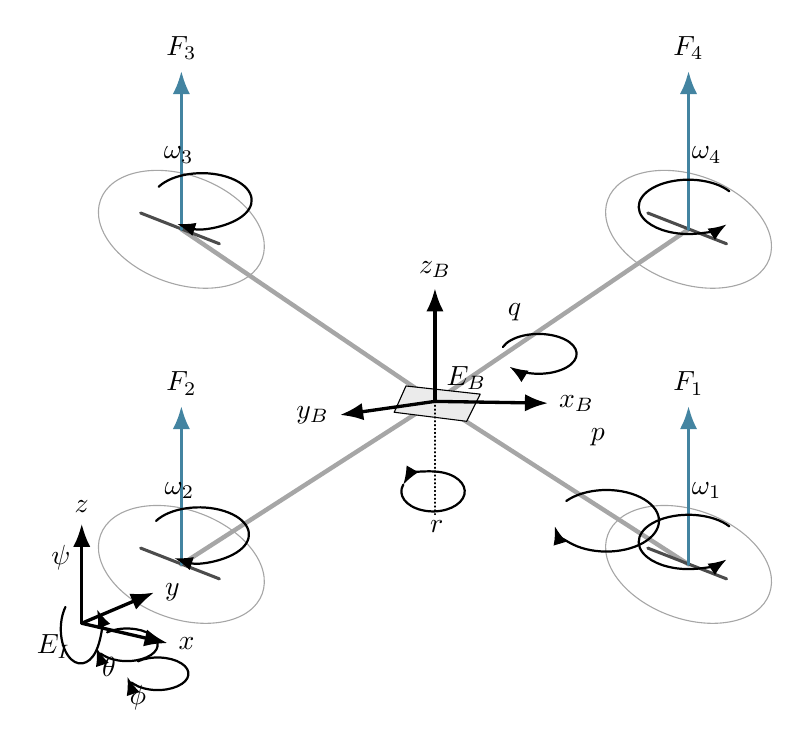
\begin{tikzpicture}[scale=1.15, >=Latex, line cap=round, line join=round]

% ------------------------------------------------
% Styles
% ------------------------------------------------
\tikzset{
    arm/.style={line width=1.6pt, gray!70},
    rotor/.style={thin, black!35},
    prop/.style={line width=1.1pt, black!70},
    axis/.style={->, very thick, black},
    force/.style={->, very thick, cyan!60!black},
    carr/.style={->, thick, black},
    lbl/.style={font=\small},
}

% ------------------------------------------------
% Main coordinates
% ------------------------------------------------
\coordinate (O)  at (0,0);
\coordinate (R3) at (-2.8, 1.9);   % top-left
\coordinate (R4) at ( 2.8, 1.9);   % top-right
\coordinate (R2) at (-2.8,-1.8);   % bottom-left
\coordinate (R1) at ( 2.8,-1.8);   % bottom-right

% ------------------------------------------------
% Arms
% ------------------------------------------------
\draw[arm] (R3)--(O)--(R1);
\draw[arm] (R2)--(O)--(R4);

% small body
\draw[fill=black!8] (-0.45,-0.12) -- (0.35,-0.22) -- (0.50,0.08) -- (-0.32,0.17) -- cycle;

% ------------------------------------------------
% Rotors and propellers
% ------------------------------------------------
\foreach \P/\ang in {R1/-20,R2/-20,R3/-20,R4/-20}{
    \draw[rotor] (\P) ellipse[x radius=0.95, y radius=0.60, rotate=\ang];
}

\draw[prop] ($(R1)+(-0.45,0.18)$)--($(R1)+(0.42,-0.16)$);
\draw[prop] ($(R2)+(-0.45,0.18)$)--($(R2)+(0.42,-0.16)$);
\draw[prop] ($(R3)+(-0.45,0.18)$)--($(R3)+(0.42,-0.16)$);
\draw[prop] ($(R4)+(-0.45,0.18)$)--($(R4)+(0.42,-0.16)$);

% ------------------------------------------------
% Thrust forces
% ------------------------------------------------
\draw[force] (R1) -- ++(0,1.75) node[above, black] {$F_1$};
\draw[force] (R2) -- ++(0,1.75) node[above, black] {$F_2$};
\draw[force] (R3) -- ++(0,1.75) node[above, black] {$F_3$};
\draw[force] (R4) -- ++(0,1.75) node[above, black] {$F_4$};

% ------------------------------------------------
% Rotor angular velocity arrows (corrected placement)
% ------------------------------------------------
% omega_1
\draw[carr] ($(R1)+(0.45,0.42)$)
    arc[start angle=35,end angle=320,x radius=0.55,y radius=0.30];
\node at ($(R1)+(0.20,0.82)$) {$\omega_1$};

% omega_2
\draw[carr] ($(R2)+(-0.28,0.48)$)
    arc[start angle=150,end angle=-120,x radius=0.55,y radius=0.30];
\node at ($(R2)+(-0.02,0.82)$) {$\omega_2$};

% omega_3
\draw[carr] ($(R3)+(-0.25,0.47)$)
    arc[start angle=150,end angle=-120,x radius=0.55,y radius=0.30];
\node at ($(R3)+(-0.03,0.82)$) {$\omega_3$};

% omega_4
\draw[carr] ($(R4)+(0.45,0.42)$)
    arc[start angle=35,end angle=320,x radius=0.55,y radius=0.30];
\node at ($(R4)+(0.20,0.82)$) {$\omega_4$};

% ------------------------------------------------
% Body frame axes
% ------------------------------------------------
\draw[axis] (O) -- ++(1.25,-0.02) node[right] {$x_B$};
\draw[axis] (O) -- ++(-1.05,-0.15) node[left] {$y_B$};
\draw[axis] (O) -- ++(0,1.25) node[above] {$z_B$};

\node[above right=1pt] at (O) {$E_B$};

% ------------------------------------------------
% Body angular rates p, q, r (corrected regions)
% ------------------------------------------------
% q near upper-right arm
\draw[carr] ($(0.75,0.60)$)
    arc[start angle=160,end angle=-140,x radius=0.42,y radius=0.22];
\node at ($(0.88,0.98)$) {$q$};

% p near lower-right arm
\draw[carr] ($(1.45,-1.10)$)
    arc[start angle=140,end angle=-170,x radius=0.58,y radius=0.34];
\node at ($(1.80,-0.40)$) {$p$};

% r below body center
\draw[carr] ($(O)+(-0.35,-0.92)$)
    arc[start angle=160,end angle=520,x radius=0.35,y radius=0.22];
\node at ($(O)+(0.02,-1.38)$) {$r$};

\draw[densely dotted] (O) -- ++(0,-1.25);

% ------------------------------------------------
% Inertial frame E_I
% ------------------------------------------------
\coordinate (I) at (-3.9,-2.45);

\node[below left=1pt] at (I) {$E_I$};

\draw[axis] (I) -- ++(0.95,-0.22) node[right] {$x$};
\draw[axis] (I) -- ++(0.80,0.34) node[right] {$y$};
\draw[axis] (I) -- ++(0,1.10) node[above] {$z$};

% psi about z-axis
\draw[carr] ($(I)+(-0.18,0.18)$)
    arc[start angle=140,end angle=395,x radius=0.22,y radius=0.38];
\node at ($(I)+(-0.23,0.72)$) {$\psi$};

% theta middle
\draw[carr] ($(I)+(0.28,-0.10)$)
    arc[start angle=130,end angle=-170,x radius=0.34,y radius=0.18];
\node at ($(I)+(0.30,-0.48)$) {$\theta$};

% phi lowest
\draw[carr] ($(I)+(0.62,-0.42)$)
    arc[start angle=130,end angle=-170,x radius=0.34,y radius=0.18];
\node at ($(I)+(0.62,-0.82)$) {$\phi$};

\end{tikzpicture}
\end{document}